\section{Methodology: Experimental Design}

\subsection{Data Source and preproccesing: 16,301 Conversations with Elderly Users}

The initial stage of this research involved the curation of a large-scale conversational corpus. The raw data comprised approximately 30,561 sessions; however, to ensure the reliability of the self-disclosure analysis, a multi-stage preprocessing pipeline was applied to refine the dataset.

\begin{enumerate}
    \item \textbf{Filtering of Ludic Interactions:} Messages categorized under the \texttt{intent == games} label (e.g., riddles, word searches) were removed. These interactions are governed by rigid game logic rather than spontaneous social exchange, making them unsuitable for studying natural self-revelation.
    \item \textbf{System Message Cleaning:} Technical artifacts, such as the automated response \texttt{(pensando...)} generated during system latency, were purged. This ensures that the subsequent Natural Language Processing (NLP) tasks are performed strictly on human and intentional bot-generated content.
    \item \textbf{Minimal Interaction Constraint:} A threshold was set to exclude sessions with fewer than five total exchanges (human-bot turns). This criterion ensures that only sessions with enough conversational "mass" to exhibit depth are included in the study.
\end{enumerate}



As a result of this process, the final dataset was reduced to \textbf{16,301 valid sessions}. For data management purposes, each session was mapped from a composite identifier \newline \texttt{'\{user\_id\}\_\{session\_id\}.csv'}. This structured approach allows for efficient feature engineering while maintaining the integrity of the original conversational flows.


Beyond the total number of sessions, the dataset comprises \textbf{2,174 unique users}. The relationship between users and their respective number of interactions provides insight into the engagement patterns of the elderly population with the AI system.

\begin{figure}[htbp]
    \centering
    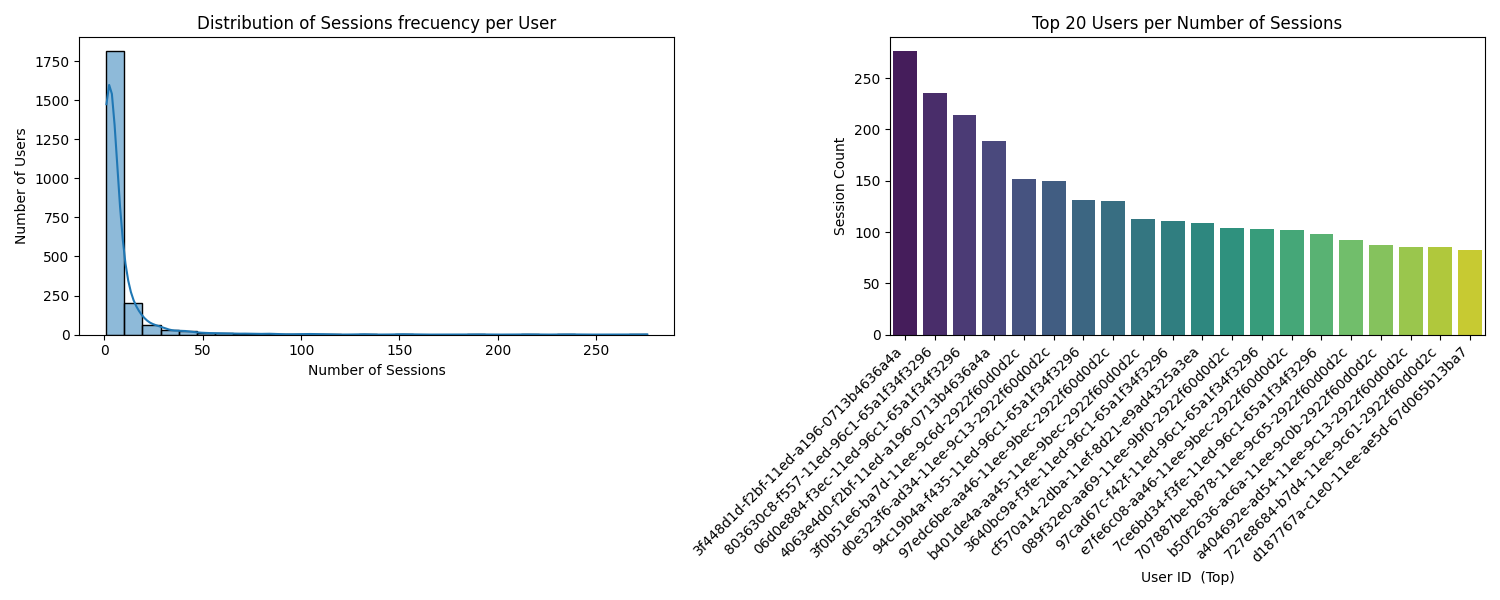
\includegraphics[width=0.8\textwidth]{images/user_dist.png}
    \caption{Distribution of the number of conversations per user (Top 20 most active users).}
    \label{fig:user_dist}
\end{figure}

As shown in Figure \ref{fig:user_dist}, there is a significant variance in user activity. This concentration of data in the most active users allows for a robust analysis of conversational depth, as these long-term interactions are more likely to transition from superficial "cliché" exchanges to more intimate layers of disclosure.

    \newpage
    \subsection{Programmatic Feature Engineering}

In addition to the semantic evaluation, a quantitative characterization of the sessions was performed through programmatic feature engineering. This process involved the extraction of objective metrics that describe the structural, temporal, and emotional dynamics of the human-computer interaction. While the semantic layers focus on \textit{what} is being said, these features provide crucial context on \textit{how} the interaction unfolds.

The engineered features can be categorized into three main groups:
\begin{itemize}
    \item \textbf{Structural and Temporal:} Metrics such as \texttt{session\_duration} and \texttt{n\_user\_interactions} quantify the level of engagement and the length of the conversational exchange.
    \item \textbf{Linguistic Complexity:} Features like \texttt{len\_user\_interactions} and \texttt{n\_proper\_nouns} serve as proxies for the richness of the discourse, where a higher density of proper nouns often correlates with the mention of specific personal entities or anecdotes.
    \item \textbf{Affective Analysis:} Sentiment scores (\texttt{pos}, \texttt{neu}, \texttt{neg}) were calculated for both the user and the bot. Comparing these allows for the assessment of emotional reciprocity, a key component in deepening social penetration.
\end{itemize}

\begin{table}[htbp]
\centering
\caption{Description of Programmatically Engineered Features.}
\label{tab:programmatic_features}
\begin{tabular}{@{}ll@{}}
\toprule
\textbf{Feature Name} & \textbf{Description}  \\ \midrule
\texttt{session\_duration} & Total duration of the session in seconds or minutes. \\
\texttt{n\_user\_interactions} & Total number of interactions initiated by the user. \\
\texttt{percentage\_user\_interactions} & User's share of interactions relative to the session total.  \\
\texttt{len\_user\_interactions} & Average length of the user's messages/inputs. \\
\texttt{n\_proper\_nouns} & Number of proper nouns detected in the conversation.\\
\texttt{user\_sent\_pos} & Positive sentiment score in the user's messages.\\
\texttt{user\_sent\_neu} & Neutral sentiment score in the user's messages. \\
\texttt{user\_sent\_neg} & Negative sentiment score in the user's messages. \\
\texttt{bot\_sent\_pos} & Positive sentiment score in the bot's responses. \\
\texttt{bot\_sent\_neu} & Neutral sentiment score in the bot's responses. \\
\texttt{bot\_sent\_neg} & Negative sentiment score in the bot's responses. \\ \bottomrule
\end{tabular}
\end{table}
    \subsection{Operationalizing Self-Disclosure Categories}

We have defined three primary categories that aggregate various conversational themes. These categories serve as proxies for the breadth and depth of the users' "social personality" layers:

\begin{itemize}
    \item \textbf{Category 1: Health and Well-being.} Focuses on the most immediate and vital concerns of the elderly population. It includes \textit{Mental and Emotional Health} as well as \textit{Physical Health and Addictions}.
    \item \textbf{Category 2: Interpersonal Relationships.} Maps the user's social circle and support system, encompassing \textit{Family Dynamics} and \textit{Affective/Romantic Relationships}.
    \item \textbf{Category 3: History and Personal Development.} Represents the deepest layers of the "onion," covering \textit{Personal Goals and Failures}, \textit{Traumas and Adversity}, and \textit{Professional Life and Career}.
\end{itemize}

\begin{table}[htbp]
\centering
\caption{Operationalized SPT Categories and Sub-themes.}
\label{tab:spt_categories}
\begin{tabular}{@{}ll@{}}
\toprule
\textbf{Main Category} & \textbf{Sub-themes / Dimensions} \\ \midrule
\textbf{C1: Health \& Well-being} & Mental Health, Emotional State, Physical Health, Addictions \\
\textbf{C2: Interpersonal Rel.} & Family Dynamics, Affective Relationships \\
\textbf{C3: Personal Development} & Goals \& Failures, Traumas \& Adversity, Career History \\ \bottomrule
\end{tabular}
\end{table}

This categorization allows the model to assign a numerical score to each session based on the presence and intensity of these topics, effectively creating a "disclosure profile" for every interaction.

    
    \subsection{LLM-Based Feature Extraction (Gemma-2-9b-it)}

The semantic characterization of the corpus was approached through three distinct experiments. These setups aim to compare how different levels of abstraction and scoring methods impact the model's ability to cluster users according to the Social Penetration Theory.

\begin{table}[htbp]
\centering
\caption{Summary of LLM-Based Feature Extraction Experiments.}
\label{tab:llm_experiments}
\begin{tabular}{@{}lp{6cm}p{4.5cm}@{}}
\toprule
\textbf{Experiment} & \textbf{Objective} & \textbf{Methodology} \\ \midrule
\textbf{4.2.3: Exp. A} & Integration of intensity and presence via \textbf{Hadamard Product}. & Rubric (0-5) $\odot$ Binary (0/1) at subcategory level. \\
\textbf{4.2.2: Exp. B} & Direct comparison of scoring granularity at the \textbf{Category level}. & Rubric vs. Binary evaluation for C1, C2, and C3. \\
\textbf{4.2.1: Exp. C} & Fine-grained analysis of \textbf{Subtopics}. & Rubric vs. Binary evaluation for individual subtopics. \\ \bottomrule
\end{tabular}
\end{table}



To ensure consistency between the computational implementation and the analytical results, a standardized nomenclature was established for the six experimental variants. These are grouped into three main categories based on their granularity (Category vs. Subtopic) and their scoring logic (Rubric, Binary, or Hadamard Fusion).

\begin{table}[htbp]
\centering
\caption{Technical nomenclature of the experiments conducted.}
\label{tab:experiment_names}
\begin{tabular}{@{}cllp{5cm}@{}}
\toprule
\textbf{Exp.} & \textbf{ID} & \textbf{Technical Name} & \textbf{Description} \\ \midrule
\textbf{A} & 1 & \texttt{rubric based hadamard fusion} & Category-level rubric scores. \\
           & 2 & \texttt{binary hadamard fusion} & Category-level scores from binary flags. \\ \midrule
\textbf{B} & 3 & \texttt{topic rubric} & Direct evaluation of the 3 main categories using a 0-5 scale. \\
           & 4 & \texttt{topic binary} & Direct presence/absence detection of the 3 main categories. \\ \midrule
\textbf{C} & 5 & \texttt{subtopic rubric} & Detailed 0-5 scoring for each specific sub-dimension. \\
           & 6 & \texttt{subtopic binary} & Presence/absence detection for each specific sub-dimension. \\ \bottomrule
\end{tabular}
\end{table}



\textbf{Experiment A} represents our primary approach, where we hypothesize that multiplying the rubric score by a binary flag (Hadamard Product) filters out low-confidence model assignments while preserving the intensity of high-quality disclosures.\\
\textbf{Experiments B and C} serve as ablation studies and validation baselines to justify the complexity of the feature engineering process.


        \subsubsection{Experiment C: Subtopics (Rubric vs Binary)}
The experimental workflow follows a bottom-up structure, beginning with \textbf{Experiment C (Subtopics)} due to a critical data dependency. This experiment serves as the foundational feature extraction layer; it is a mathematical prerequisite to obtain granular scores for each specific sub-dimension before executing higher-level operations.

The evaluation of subtopics was operationalized through a zero-shot/few-shot hybrid prompt. This prompt defines the semantic boundaries for each of the seven subtopics and establishes a rigorous scoring rubric. Below is the technical implementation of the system prompt used:

\begin{lstlisting}[language=json, caption={System Prompt for Subtopic Feature Extraction.}, label={lst:prompt_subtopics}, frame=single, basicstyle=\small\ttfamily, breaklines=true]
<start_of_turn>user
You are a text analysis system. Your goal is to quantify the level of self-disclosure in a predefined list of topics:
- Health (Mental/Physical)
- Relationships (Family/Affective)
- Personal History (Goals, Traumas, Career)

Analyze the [MESSAGES TO EVALUATE] and assign a score (0-5) to EACH topic. 
Response must be ONLY a valid JSON object.

# EVALUATION SCALE (0-5)
* 0: No Mention.
* 1: Impersonal Mention (General talk).
* 2: Vague Personal Mention (General identification).
* 3: Specific Action Disclosure (Concrete habits/actions).
* 4: Detailed Disclosure (Sharing reasoning/beliefs).
* 5: Deep Disclosure (Vulnerability, impact, deep emotions).

# EXPECTED JSON FORMAT
{
  "mental_emotional_health": Int,
  "physical_health_addictions": Int,
  "family_dynamics": Int,
  "affective_relationships": Int,
  "personal_goals_failures": Int,
  "traumas_adversities": Int,
  "professional_career": Int
}

[MESSAGES TO EVALUATE]: 
<end_of_turn>
\end{lstlisting}

For the binary variant of Experiment C, the model's instructions were simplified to a detection task. The prompt explicitly forbids intermediate values, forcing a strictly boolean output (0 or 1). This reduction in dimensionality serves to minimize variance and provide a high-confidence indicator of thematic occurrence.

\begin{lstlisting}[language=json, caption={System Prompt for Binary Subtopic Detection.}, label={lst:prompt_binary}, frame=single, basicstyle=\small\ttfamily, breaklines=true]
<start_of_turn>user
You are a high-precision text classification system. Your task is to detect the PRESENCE or ABSENCE of specific self-disclosure topics in the provided text.

Analyze the [MESSAGES TO EVALUATE] and assign a value of 1 if the topic is mentioned (regardless of its depth) and 0 if it is not mentioned at all.
Your response must be ONLY a valid JSON object.

# TOPICS TO DETECT
- mental_emotional_health
- physical_health_addictions
- family_dynamics
- affective_relationships
- personal_goals_failures
- traumas_adversities
- professional_career

# DETECTION RULES
* 0: There is no trace of the topic in the text.
* 1: The topic is present in the text (even if vaguely mentioned).

# EXPECTED JSON FORMAT
{
  "mental_emotional_health": 0 or 1,
  "physical_health_addictions": 0 or 1,
  "family_dynamics": 0 or 1,
  "affective_relationships": 0 or 1,
  "personal_goals_failures": 0 or 1,
  "traumas_adversities": 0 or 1,
  "professional_career": 0 or 1
}

[MESSAGES TO EVALUATE]:
<end_of_turn>
\end{lstlisting}



        
        \subsubsection{Experiment A: Rubric-Based vs. Binary Scoring via Hadamard Product}

The hadamard product is used to merge the qualitative depth of the scores.

Given two vectors of dimension $n$, $\mathbf{R}$ (representing rubric scores) and $\mathbf{B}$ (representing binary inclusion to category), the Hadamard product $\odot$ is defined as:
\begin{equation}
    \mathbf{F} = \mathbf{R} \odot \mathbf{B}
\end{equation}

Where each component of the resulting fused vector $\mathbf{F}$ is calculated as:
\begin{equation}
    f_{i} = r_{i} \times b_{i} \quad \text{for  } i = 1, \dots, n
\end{equation}

In matrix-vector form, the operation is represented as:
\begin{equation}
    \begin{bmatrix} r_1 \\ r_2 \\ \vdots \\ r_n \end{bmatrix} \odot \begin{bmatrix} b_1 \\ b_2 \\ \vdots \\ b_n \end{bmatrix} = \begin{bmatrix} r_1 \cdot b_1 \\ r_2 \cdot b_2 \\ \vdots \\ r_n \cdot b_n \end{bmatrix}
\end{equation}

This approach implements a \textit{gating mechanism} where the binary vector $\mathbf{B}$ validates the presence of the category. 

\begin{lstlisting}[language=Python, caption={Mapping of Subtopics to SPT Categories.}, label={lst:mapping_categories}, frame=single, basicstyle=\small\ttfamily]
category_mapping = {
    'Category 1: Health and Well-being': [
        'mental_emotional_health', 
        'physical_health_addictions'
    ],
    'Category 2: Interpersonal Relationships': [
        'family_dynamics', 
        'affective_relationships'
    ],
    'Category 3: Personal History and Development': [
        'personal_goals_failures', 
        'traumas_adversities', 
        'professional_career'
    ]
}
\end{lstlisting}


        
        \subsubsection{Experiment B: Direct Category Evaluation (Rubric vs Binary)}

The rubric-based prompt for Experiment B provides the model with a nuanced scale to differentiate between impersonal mentions and deep emotional vulnerability. This allows for a direct comparison with the aggregated results of Experiment A to determine if "direct inference" leads to a loss of granularity.

\begin{lstlisting}[language=json, caption={System Prompt for Direct Category Rubric Evaluation.}, label={lst:prompt_exp_b_rubric}, frame=single, basicstyle=\small\ttfamily, breaklines=true]
<start_of_turn>user
You are a text analysis system. Your goal is to quantify the level of self-disclosure in a predefined list of categories focused on lived experiences and the author's inner world.

Analyze the [MESSAGES TO EVALUATE] and assign a score (0-5) to EACH category.
Response must be ONLY a valid JSON object.

# CATEGORIES TO EVALUATE
* 'Category 1: Health and Well-being': Includes physical, mental, and emotional health.
* 'Category 2: Interpersonal Relationships': Includes family dynamics and affective relationships.
* 'Category 3: Personal History and Development': Includes goals, failures, traumas, and career.

# EVALUATION SCALE (0-5)
* 0: No Mention.
* 1: Impersonal Mention (General discussion, no personal link).
* 2: Vague Personal Mention (General identification or labels).
* 3: Specific Action Disclosure (Concrete habits or specific actions)
* 4: Detailed Disclosure (Reasoning, beliefs, or specific data).
* 5: Deep Disclosure (Vulnerability, fear, or profound personal impact).

# EXPECTED JSON FORMAT
{
    "Category 1: Health and Well-being": Int,
    "Category 2: Interpersonal Relationships": Int,
    "Category 3: Personal History and Development": Int
}

[MESSAGES TO EVALUATE]: 
<end_of_turn>
\end{lstlisting}

        
The prompt for Experiment B (Binary) instructs the model to act as a high-level classifier. Unlike the subtopic prompt, this version requires the LLM to perform an internal aggregation, considering various aspects (e.g., physical health and emotional state) under a single categorical label.

\begin{lstlisting}[language=json, caption={System Prompt for Direct Category Binary Evaluation.}, label={lst:prompt_exp_b}, frame=single, basicstyle=\small\ttfamily, breaklines=true]
<start_of_turn}user
You are a text analysis system. Your goal is to quantify the level of self-disclosure in a predefined list of broad categories:
- Category 1: Health and Well-being (Mental, emotional, and physical health)
- Category 2: Interpersonal Relationships (Family dynamics, affective relationships).
- Category 3: Personal History and Development (Goals, failures, traumas, career).

Analyze the [MESSAGES TO EVALUATE] and assign a 0 or 1 to EACH category.
Response must be ONLY a valid JSON object.

# BINARY EVALUATION SCALE (0-1)
* 0: No Mention or Not Relevant: The topic is not mentioned or not linked personally.
* 1: Specific Action/Deep Disclosure: The author reveals a concrete habit, action, or reflects deeply on the topic.

# EXPECTED JSON FORMAT
{
    "Category 1: Health and Well-being": 0 or 1,
    "Category 2: Interpersonal Relationships": 0 or 1,
    "Category 3: Personal History and Development": 0 or 1
}

[MESSAGES TO EVALUATE]: 
<end_of_turn>
\end{lstlisting}


    \subsection{Clustering Strategy}
        \subsubsection{Implementation of the K-Means Algorithm}
        \subsubsection{Justification of the N+1 Cluster Architecture}